\begin{recipe}
[ %
	preparationtime = {\SI{5}{\hour}},
	bakingtime={\SI{3}{\hour}},
	bakingtemperature={\protect\bakingtemperature{topbottomheat=\SIrange{250}{300}{\fahrenheit} (\SIrange{120}{150}{\celsius})}},
	portion = {\portion{3--4}},
	source = {BrainStew}
    ]{Duck Confit Tacos}

	\begin{figure}[p]
		\centering
		\makebox[\textwidth][c]{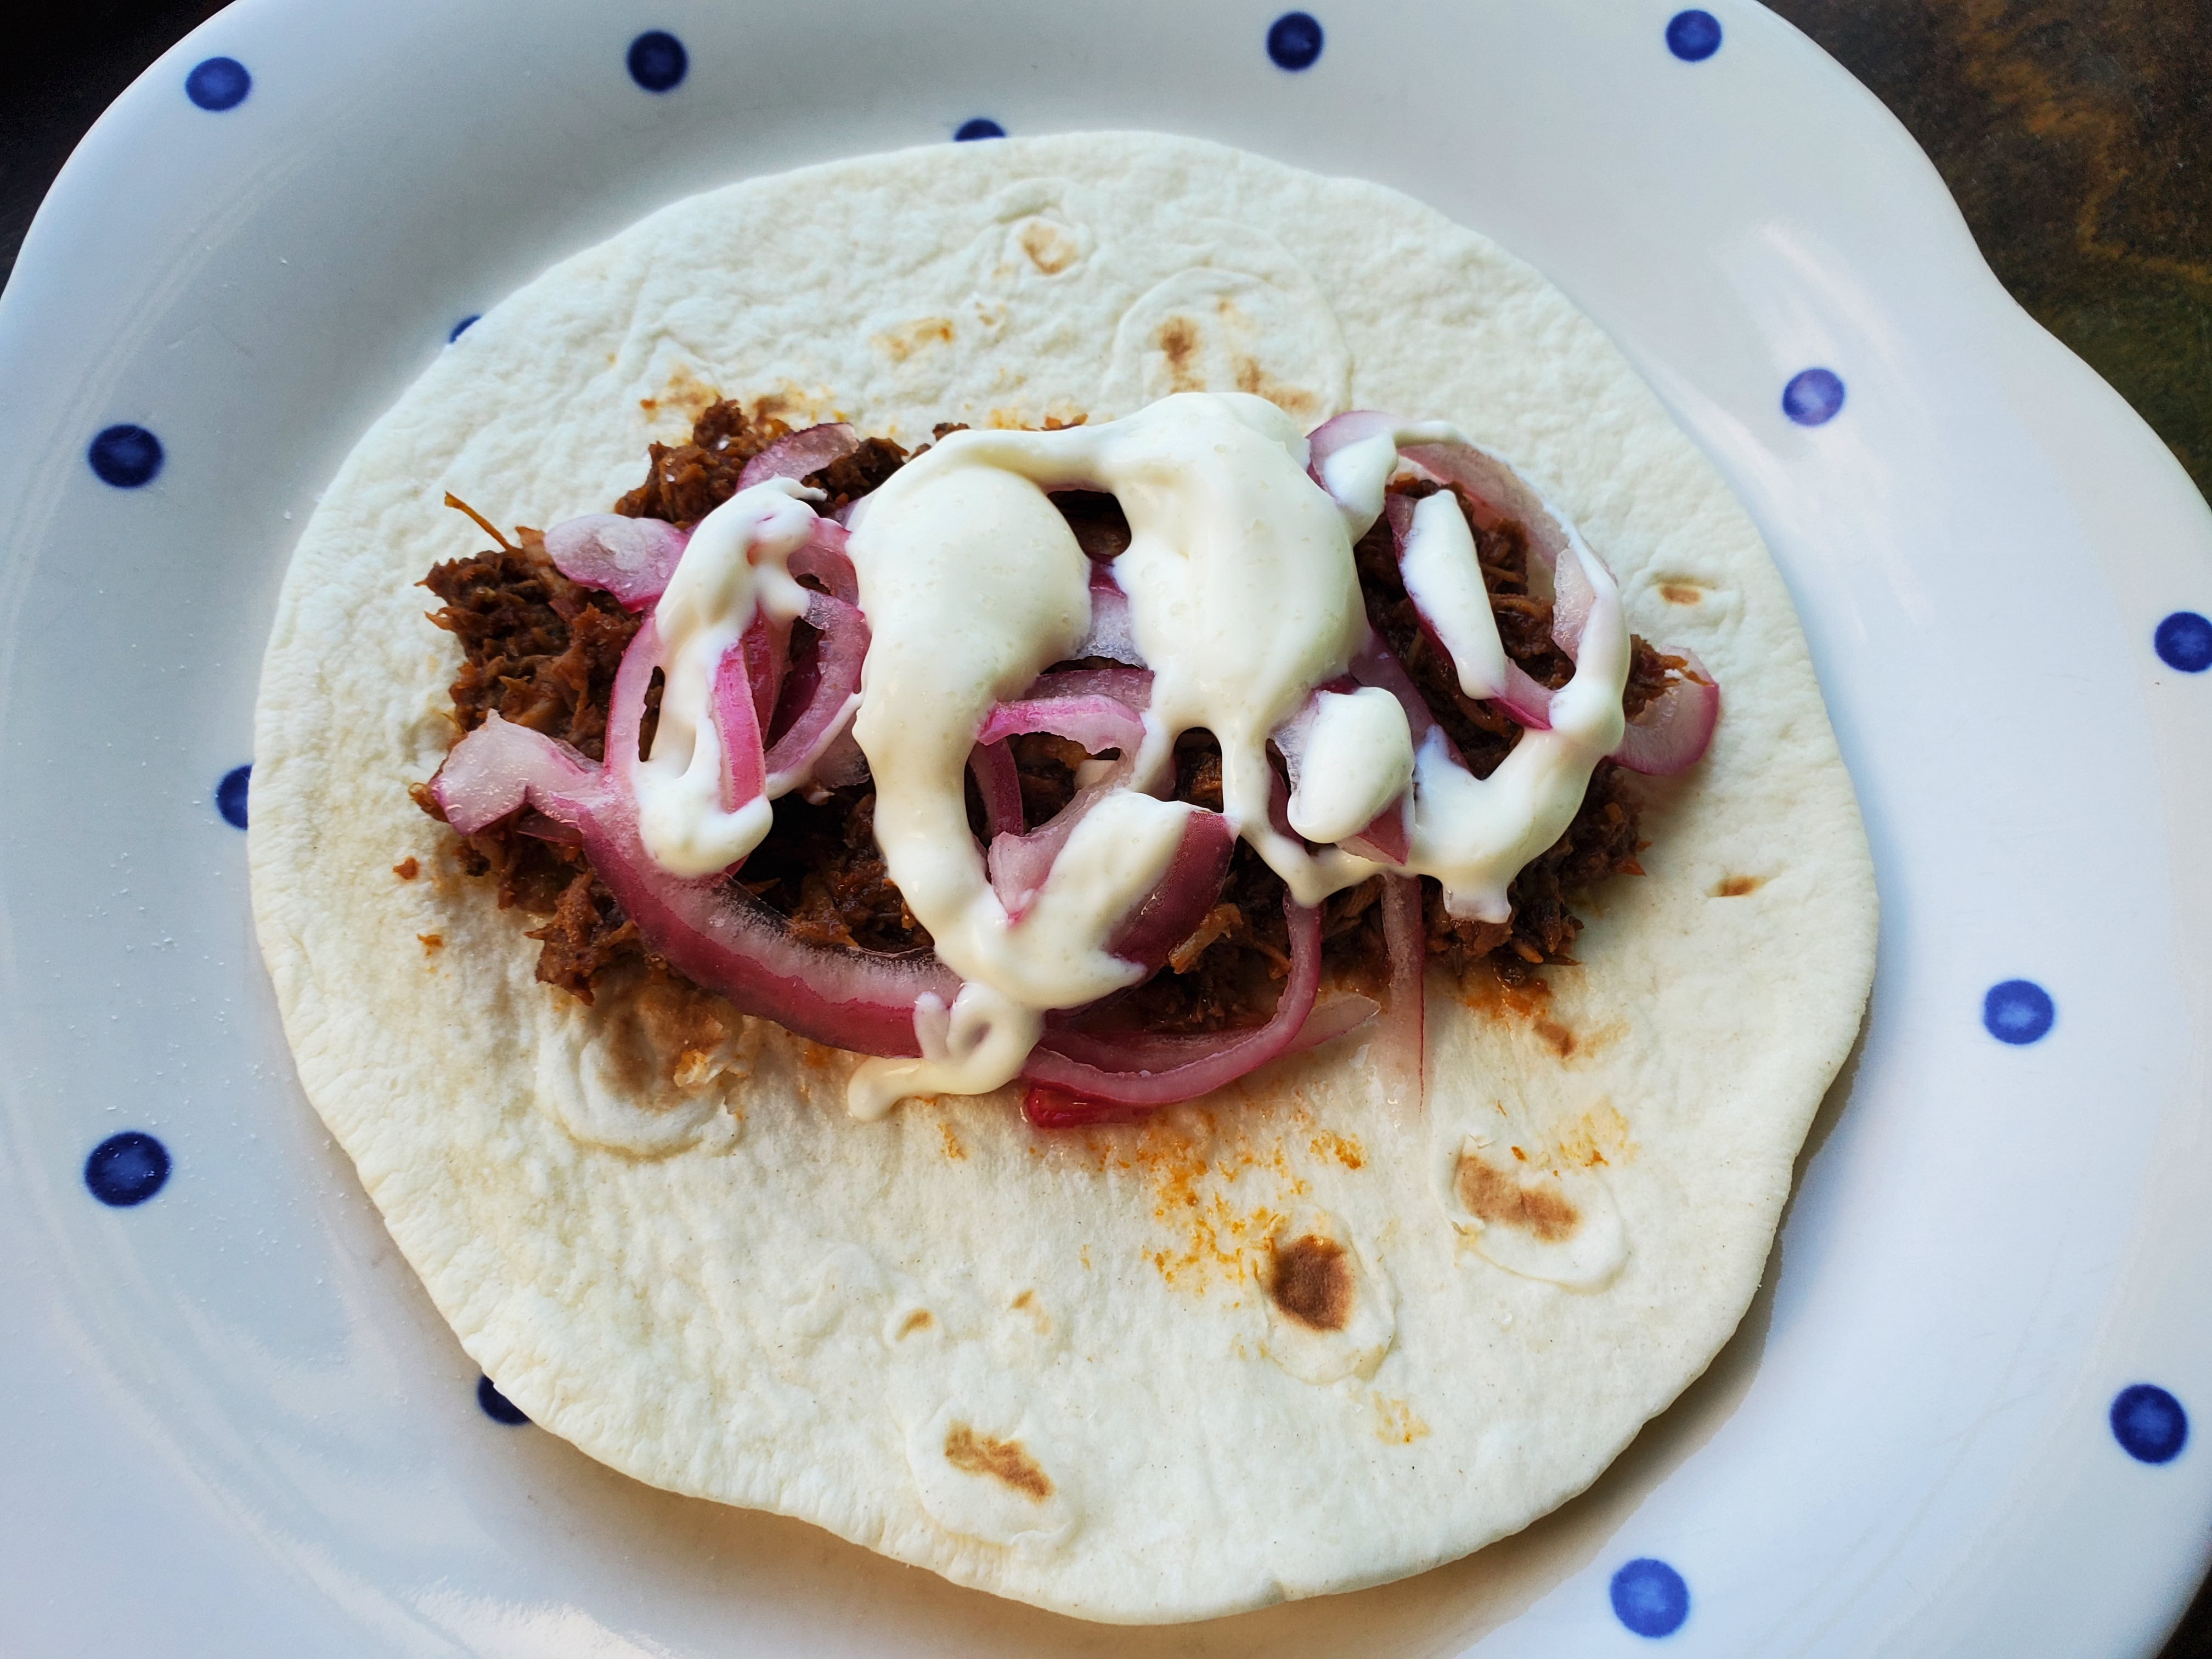
\includegraphics[height=\textheight]{duck_confit_tacos/20200501_181903.jpg}}
	\end{figure}

    \introduction{
    	You can replace ancho chilies with guajillo, or any other large, smokey dried chilies.

    	If you don't have rice vinegar you can substitute white vinegar or white wine vinegar.
	}

	\ingredients[23]{
		1 & Duck \\
		& Garlic \\
		& Onion or shallots \\
		& Herbs and spices \\
		& Small corn or flour tortillas, soft \\
		\multicolumn{2}{c}{\textbf{Pickled Onions}} \\
		1 & Red onion, thinly sliced \\
		\SI{2}{\teaspoon} & Salt (split, you will use half and half) \\
		\SI{1/2}{\cup} & Sugar \\
		\SI{1/2}{\cup} & Boiling/very hot water \\
		\SI{1x1/3}{\cup} & Rice vinegar \\
		\multicolumn{2}{c}{\textbf{The Filling}} \\
		5 & Dried ancho chilies \\
		\SI{2}{cups} & Boiling water \\
		\SI{1/2}{\cup} & Dried cherries \\
		\SI{6}{cloves} & Garlic cloves, peeled \\
		\SI{1}{\teaspoon} & Dried oregano, preferably Mexican \\
		\SI{1}{\teaspoon} & Black peppercorns \\
		\SI{1/2}{\teaspoon} & Cumin seeds \\
		\SI{1/4}{\cup} & White-wine vinegar \\
		\SI{1}{\teaspoon} & Sea salt \\
		& Some neutral oil \\
%		Confit duck
		\multicolumn{2}{c}{\textbf{Lime Crema}} \\
		\SI{1/2}{\cup} & Sour cream or creme fresh \\
		\SI{1/3}{\cup} & Lime juice
	}

	\preparation{

		\textbf{\large Part 1: Confit Your Duck}

		\step Get a whole duck, preferably fresh if possible. If bought frozen, let it fully defrost before attempting to confit the duck.

		\step Remove the breast sections, wings (if using, they are not very meaty), and thighs/legs and any other meaty bits.

		\step Take any remaining skin or fat left on the carcass and remove it. Dice the skin and fat down small and throw it in a sauce-pan. Return to this later.

		\step Put your duck meat into a container where it packs tightly, but with sides higher than the meat reaches and that is oven safe. Season the duck with salt and pepper and sandwich some garlic cloves, onion or shallot pieces, fresh herbs, and other flavor-enhancers between the meat layers. Let this sit in the fridge for as long as possible (ideally overnight) before beginning the cooking process.

		\step While the duck is resting, heat your pan of duck fat and skin, making sure to stir constantly\footnote{If you're worried about burning, you can add a bit of water at the start and boil it off as the fat starts to render out.}. The fat will render out of the pieces and eventually you should have golden brown duck cracklings floating in hot duck fat. Drain the cracklings and season if desired. They make a delicious snack! You can also use them as a topping for your tacos (see below continuation of this recipe). Reserve the oil in a heat proof container.

		\step Once the duck has rested, remove the herbs and other seasonings. Pack the duck meat in tightly and cover with the duck fat. If the duck fat has solidified, gently warm it before using. Ideally the duck fat will cover all of the meat. If it does not, either supplement with store bought duck fat, or with a neutral oil.

		\step Cook at \SIrange{250}{300}{\fahrenheit} (\SIrange{120}{150}{\celsius}), or whatever heat just barely gets the oil bubbling. Cook for at least \SI{3}{\hour} and remove the meat from the oil before it solidifies again. Pull the meat off of the bones carefully, and keep the duck fat if desired for future Confit cookings.

		\textbf{\large Part 2: The Tacos}

		\step Make the pickled onions. First, rub the onions with half of the salt and let sit for \SI{10}{\minute}. While they sit, mix everything but the vinegar together and stir until the solids dissolve. Once everything is dissolved, add the vinegar.

		\step After the 10 minutes, pat off excess moisture and salt from the onions with a paper towel and put in the brine. Soak for \SI{1}{\hour}. They can also be stored for months in the brine.

		\step Prepare the chilies and cherries. Toast the chilies in a dry pan over medium heat for \SI{5}{\minute} to release oils.

		\step Pour \SI{2}{cups} of boiling water over them and let soak for \SI{15}{\minute}. Also soak the cherries in some warm water as the chilies soak.

		\step Make the chili paste. Strain the chilies (reserving the liquid) and the cherries (don't save this liquid). Throw everything but the neutral oil and duck into a food processor. Blend until you get the consistency of tomato paste or chunky mashed potatoes. Add that leftover chili water as needed to get to the right thickness.

		\step Finish filling. Warm your duck confit to room temperature and break/shred into chunks. Heat about \SI{2}{\tablespoon} of your neutral oil in a pan, ideally cast iron or other non-stick style. Depending on the amount of duck confit you have, add around \SI{1/2}{\cup} of the chili paste to the pan and heat until fragrant.

		\vspace{1em}

		\step Add duck and coat. If you need additional paste to coat the duck (or to add the correct amount of heat/flavor desites), add it a teaspoon at a time and let heat up before tasting again and adjusting.

		\step Assemble tacos. Place duck on taco (optionally on a bed of greens either with or without the taco shell), drizzle with lime crema, top with onions, and sea salt (if desired).
	}

\end{recipe}